\title{Aula 10 - Funções Hash}

\author{Prof. Gabriel Rodrigues Caldas de Aquino}

\institute
{
    Instituto de Computação \\
    Universidade Federal do Rio de Janeiro\\
    gabrielaquino@ic.ufrj.br% Your institution for the title page
}
\date{Compilado em: \\ \today} % Date, can be changed to a custom date

%----------------------------------------------------------------------------------------
%    PRESENTATION SLIDE
%----------------------------------------------------------------------------------------



\begin{frame}
    % Print the title page as the first slide
    \titlepage
\end{frame}

\begin{frame}{Funções de Hash}
    \begin{itemize}
        \item Uma função de hash aceita uma mensagem de tamanho variável $M$ como entrada.
        \item Produz um valor de tamanho fixo $h = H(M)$.
        \item O valor $h$ é chamado de \textbf{hash} ou \textbf{digest}.
    \end{itemize}
\textbf{Propriedades Desejáveis de Hash}
    \begin{itemize}
        \item A saída deve parecer \textbf{aleatória} e estar \textbf{uniformemente distribuída}.
        \item Uma pequena mudança em $M$ altera, com alta probabilidade, muitos bits de $h$.
        \item Principal objetivo: \textbf{integridade de dados}.
        \item Exemplo: se qualquer bit de $M$ for alterado, o hash $H(M)$ também mudará.
    \end{itemize}
\end{frame}

\begin{frame}{Função de Hash Criptográfica}
    \begin{itemize}
        \item Tipo especial de função de hash usada em aplicações de segurança.
        \item Deve ser \textbf{computacionalmente inviável} de quebrar com eficiência maior que força bruta.
        \item Usada para verificar se os dados foram alterados.
    \end{itemize}
\textbf{Propriedades de uma Função de Hash Criptográfica}
    \begin{itemize}
        \item \textbf{Mão única (one-way):}  
        Dado um hash $h$, é inviável encontrar uma mensagem $M$ tal que $H(M) = h$.
        \item \textbf{Livre de colisão (collision-free):}  
        É inviável encontrar duas mensagens $M_1$ e $M_2$ tais que $H(M_1) = H(M_2)$.
    \end{itemize}
\end{frame}

\begin{frame}{Preenchimento em Funções de Hash}
    \begin{itemize}
        \item Funções de hash processam mensagens em blocos de tamanho fixo.
        \item Quando a mensagem não é múltiplo do tamanho do bloco, adiciona-se \textbf{preenchimento} (padding).
        
        \begin{itemize}
            \item Mensagem preenchida até se tornar um múltiplo de um tamanho fixo (ex: 1024 bits). 
        \end{itemize}
     
        \item O preenchimento inclui o \textbf{tamanho original da mensagem} em bits.
        \begin{itemize}
          \item \textbf{Objetivo:} dificultar que um atacante crie uma mensagem alternativa com o mesmo hash.
        \end{itemize}

        \item Garante que cada mensagem de tamanho diferente resulte em um hash único e seguro.
    \end{itemize}


\end{frame}

\begin{frame}{Preenchimento em Funções de Hash}

    \begin{center}
        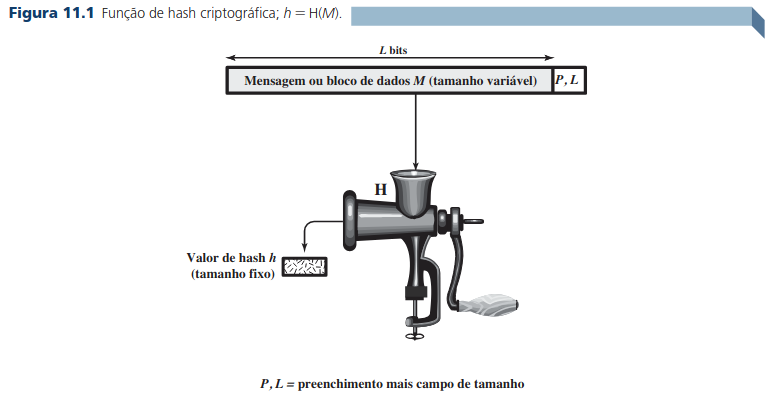
\includegraphics[width=0.8\textwidth]{Figuras/Hash-moedor.png}
    \end{center}
\end{frame}



\begin{frame}{Aplicações de Funções de Hash Criptográficas}
\textbf{Uso do Hash}:

\begin{itemize}
        \item Ela é usada em diversas aplicações de segurança e protocolos da Internet. 
    \item Talvez o hash seja o algoritmo criptográfico mais versátil.  
 
\end{itemize}

\medskip
Uso onde a Hash é empregada:

\begin{itemize}
  \item Autenticação de mensagem
  \item Assinaturas digitais
  \item Arquivo de senha de mão única
  \item Detecção de intrusão e detecção de vírus
  \item Função pseudoaleatória (PRF) 
  \item Gerador de número pseudoaleatório (PRNG)
\end{itemize}
\end{frame}


\begin{frame}{Autenticação de Mensagem}
\begin{itemize}

    \item Autenticação de mensagem é um mecanismo usado para verificar a integridade de uma mensagem

    \item Garante que os dados recebidos estão exatamente como foram enviados, sem modificação, inserção, exclusão ou repetição.  


    \item Em muitos casos, também é exigido que a identidade declarada do emissor seja validada.  

    \item Em muitas aplicações, o valor gerado pelo Hash  é chamado de \textbf{resumo de mensagem} (ou \textit{digest}, em inglês).

    
\end{itemize}
\end{frame}

\begin{frame}{Autenticação de mensagem}
A essência do uso de uma função de hash para autenticação de mensagem é a seguinte: 

\begin{enumerate}
    \item O emissor calcula um valor de hash como função dos bits da mensagem.
    \item O emissor transmite a mensagem junto com o valor de hash.
    \item O receptor recalcula o valor de hash sobre a mensagem recebida.
    \item O receptor compara o valor calculado com o valor recebido.
\end{enumerate}

\textbf{Se houver divergência}, o receptor sabe que a mensagem (ou o valor de hash) foi alterada.
\end{frame}

\begin{frame}{Autenticação básica}

\centering
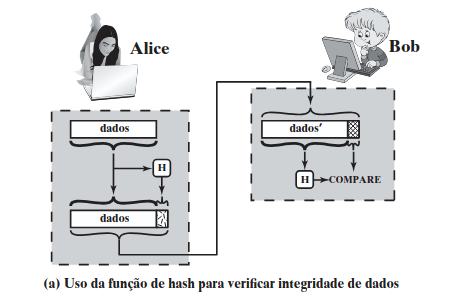
\includegraphics[width=0.6\linewidth]{Figuras/autenticacao-basica.png}

\begin{block}{Pergunta}
Qual o problema neste cenário?
\end{block}
\end{frame}

\begin{frame}{Autenticação básica - Problema}

\centering
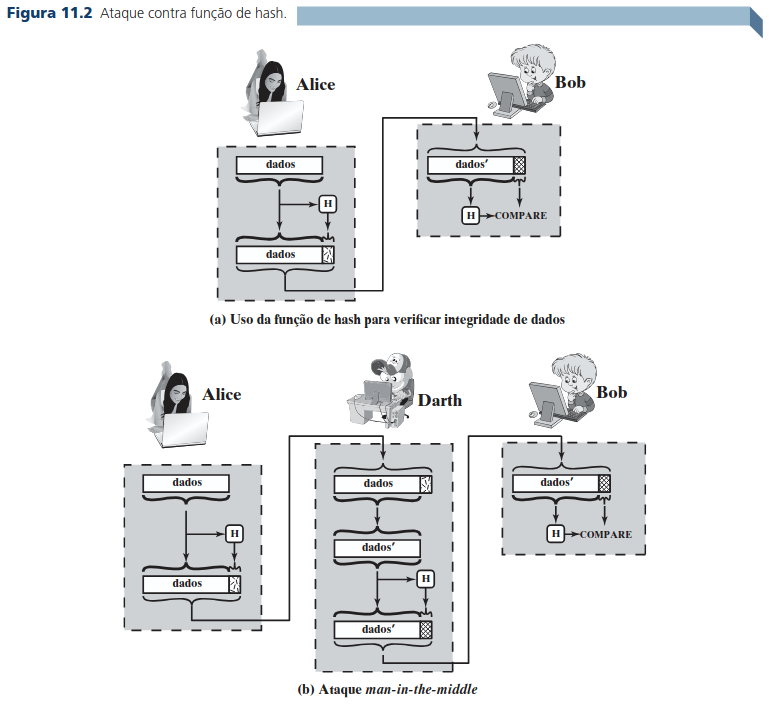
\includegraphics[width=0.6\linewidth]{Figuras/mitm-autenticacao-hash.png}


\end{frame}


\begin{frame}{Proteção do valor de hash}
A função de hash precisa ser \textbf{transmitida de forma segura}.  

\medskip

\begin{itemize}
    \item Se um adversário \textbf{alterar ou substituir} a mensagem, não deve ser viável alterar também o valor de hash para enganar o receptor.
    \item Exemplo de ataque: 
    \begin{enumerate}
        \item Alice transmite dados com o hash 
        \item Darth intercepta, altera a mensagem e calcula um novo hash
        \item Bob recebe sem perceber a modificação.
    \end{enumerate}
    \item Para impedir esse ataque, \textbf{o valor de hash gerado por Alice precisa ser protegido}.
\end{itemize}

\begin{block}{Pergunta}
    Como podemos proteger o Hash nesse cenário?
\end{block}
\end{frame}

\begin{frame}{Métodos de proteção da Hash}
    \begin{itemize}
        \item Método A: Autenticação com hash + cifragem simétrica
        \item Método B: Cifrando o hash com cifragem simétrica
        \item Método C: Mensagem com Hash e Valor Secreto
        \item Método D: Mensagem com Hash mais Valor Secreto com confidencialidade
    \end{itemize}
    
\end{frame}

\begin{frame}{Método A: Autenticação com hash + cifragem simétrica}
    \begin{itemize}
        \item Mensagem mais o código de hash concatenado \textbf{são encriptados} usando a encriptação simétrica.
        \item Como somente A e B compartilham a chave secreta, a mensagem deverá ter vindo de A e sem alteração.
        \item O código de hash oferece a estrutura ou redundância exigida para conseguir a autenticação.
        \item Como a encriptação é aplicada à mensagem inteira mais o código de hash, a confidencialidade também é fornecida.
    \end{itemize}

    \centering
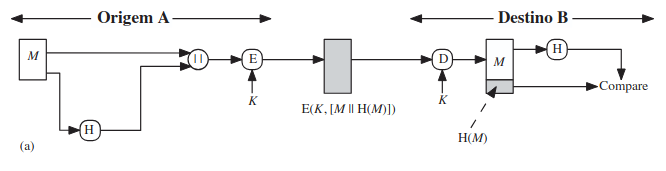
\includegraphics[width=0.7\linewidth]{Figuras/esquema1-hash.png}
\end{frame}

\begin{frame}{Método B: Cifrando o hash com cifragem simétrica}
    \begin{itemize}
        \item Somente o código de hash é encriptado, usando a encriptação simétrica. 
        \item Isso reduz o peso do processamento para as \textbf{aplicações que não exigem confidencialidade}.

    \end{itemize}

    \centering
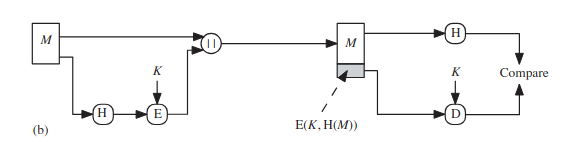
\includegraphics[width=0.7\linewidth]{Figuras/esquema2-hash.png}
\begin{block}{Pergunta}
    Qual o motivo de passar a mensagem em texto plano?
\end{block}
\end{frame}

\begin{frame}{Vantagens do Uso de Hash mas sem a cifragem da mensagem}
    \begin{itemize}
        \item Quando a \textbf{confidencialidade não é exigida}:
        \begin{itemize}
            \item usar apenas hash (método com valor secreto) requer menos cálculos que cifrar a mensagem inteira.
            \item O software de encriptação é relativamente lento, especialmente com fluxo constante de mensagens.
            \item Custos de hardware de encriptação podem ser altos; chips de baixo custo existem, mas cada nó precisa ter capacidade.
        \end{itemize} 
    \end{itemize}

    \begin{block}{Exemplo desse cenário}
        \href{https://www.linuxmint.com/edition.php?id=322}{\textcolor{blue}{Baixando a .iso do Linux Mint e verificando com GPG}}
        
    \end{block}
\end{frame}

\begin{frame}{O que o GPG faz com esses dois arquivos?}

\textbf{Comando:}
\begin{block}{}
\texttt{gpg --verify sha256sum.txt.gpg sha256sum.txt}
\end{block}

\textbf{Etapas realizadas pelo GPG:}
\begin{enumerate}
    \item Lê a assinatura digital contida em \texttt{sha256sum.txt.gpg}.
    \item Calcula o hash real do conteúdo atual de \texttt{sha256sum.txt}.
    \item Compara o hash calculado com o hash assinado.
    \begin{itemize}
        \item Se forem \textbf{iguais}: a assinatura é válida (\texttt{Good signature}).
        \item Se forem \textbf{diferentes}: a assinatura falha (\texttt{BAD signature}).
    \end{itemize}
\end{enumerate}

\end{frame}


\begin{frame}{Método C: Mensagem com Hash e Valor Secreto}
    \begin{itemize}
        \item Usar apenas uma função de hash, sem cifragem, para autenticação de mensagem.
        \item Ambas as partes compartilham um valor secreto comum: $S$.
        \item Funcionamento:
        \begin{enumerate}
            \item Emissor (A) calcula o hash sobre a concatenação da mensagem e do segredo: $H(M \,\|\, S)$.
        \item O valor de hash resultante é anexado à mensagem e enviado a B.
        \item Receptor (B), possuindo $S$, recalcula o hash para verificar a integridade e autenticidade. 
        \end{enumerate}
        
        \item Como $S$ não é enviado, um adversário não consegue modificar a mensagem nem gerar mensagens falsas.
    \end{itemize}

    \centering
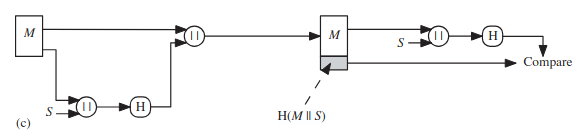
\includegraphics[width=0.7\linewidth]{Figuras/esquema3-hash.png}
\end{frame}





\begin{frame}{Código de Autenticação de Mensagem (MAC)}
\textbf{Método C é a base do HMAC - Hash Based Message Authentication Code}
    \begin{itemize}
        \item A autenticação de mensagem normalmente é alcançada usando um \textbf{MAC} (Message Authentication Code), também chamado de função de hash chaveada.
        \item MACs são usados entre duas partes que compartilham uma \textbf{chave secreta} para autenticar informações trocadas.
        \item A função MAC recebe como entrada a chave secreta e um bloco de dados, produzindo um valor de hash (\textbf{MAC}) associado à mensagem.
        \end{itemize}

\end{frame}
\begin{frame}{Código de Autenticação de Mensagem (MAC)}
    \begin{itemize}
        \item Para verificar integridade, aplica-se novamente a função MAC sobre a mensagem e compara-se com o MAC recebido.
        \item Um invasor que altere a mensagem não poderá gerar o MAC correto sem conhecer a chave secreta.
        \item A verificação também garante autenticidade: apenas a parte que conhece a chave secreta pode ter gerado o MAC.
    \end{itemize}


\end{frame}

\begin{frame}{Método D: Mensagem com Hash mais Valor Secreto com confidencialidade}
    \begin{itemize}
        \item A \textbf{confidencialidade} pode ser acrescentada à abordagem do método anterior encriptando a mensagem inteira mais o código de hash
    \end{itemize}

    \centering
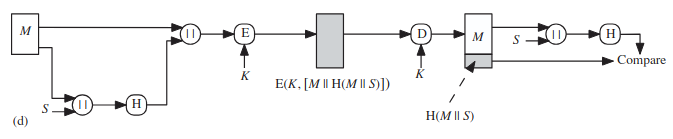
\includegraphics[width=0.7\linewidth]{Figuras/esquema4-hash.png}

\begin{block}{Cenário}
    Esse cenário mostra exatamente um canal criptografado com a autenticacao da mensagem, igual na VPN!
\end{block}
\end{frame}

\begin{frame}{Assinaturas Digitais}
    \begin{itemize}
        \item \textbf{Usa Chave pública e privada}
        \item Assinatura digital é uma aplicação importante, similar à autenticação de mensagem.
        \item O valor de hash da mensagem é encriptado com a \textbf{chave privada} do usuário.
        \item Qualquer pessoa que conheça a \textbf{chave pública} do usuário pode verificar a integridade da mensagem associada à assinatura.
        \item Um invasor que tente alterar a mensagem precisaria conhecer a chave privada do usuário.
    \end{itemize}


        \centering
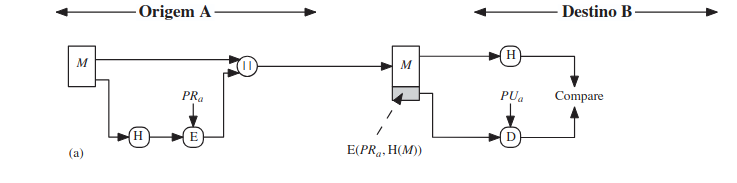
\includegraphics[width=0.7\linewidth]{Figuras/hash-certificado-digtal1.png}

\textbf{Esse caso é exatamente o caso do hash da iso do Linux Mint!}
\end{frame}

\begin{frame}{Assinaturas Digitais com Confidencialidade}
    \begin{itemize}
        \item Se, além da assinatura digital, o que se procura é confidencialidade, então a mensagem mais o código
hash encriptado com a chave privada pode ser encriptado usando uma chave secreta simétrica. Essa é
uma técnica comum.

    \end{itemize}


        \centering
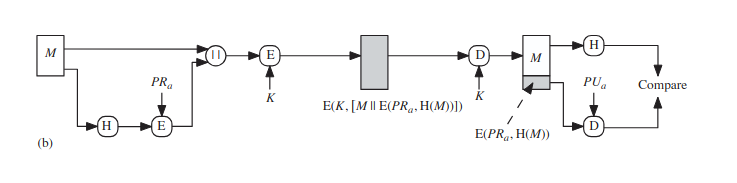
\includegraphics[width=0.7\linewidth]{Figuras/hash-certificado-digtal2.png}
\end{frame}


\begin{frame}{Arquivos de Senha de Mão Única}
    \begin{itemize}
        \item Funções de hash são usadas para criar arquivos de senha de \textbf{mão única}.
        \begin{itemize}
            \item No linux usa-se o /etc/shadow
        \end{itemize}
        \item Em vez de armazenar a senha real, o sistema operacional armazena o \textbf{hash da senha}.
        \item Assim, mesmo que um hacker acesse o arquivo, a senha real não pode ser recuperada.
        \item Processo de autenticação:
        \begin{enumerate}
            \item O usuário fornece a senha 
            \item O sistema compara o \textbf{hash informado} com o hash armazenado.
        \end{enumerate} 
        \item Este método é amplamente usado na maioria dos sistemas operacionais.
    \end{itemize}
\end{frame}

\begin{frame}{Detecção de Intrusão e Vírus com Hash}
    \begin{itemize}
        \item Funções de hash podem ser usadas para \textbf{detecção de intrusão} e \textbf{detecção de vírus}.
        \item Armazene $H(F)$ para cada arquivo em um sistema e guarde os valores de hash de forma segura.
        \item Posteriormente, verifique se um arquivo foi modificado recalculando $H(F)$.
        \item Um intruso precisaria alterar $F$ sem alterar $H(F)$ para evitar detecção, o que é computacionalmente inviável.


        
    \end{itemize}

   \textbf{Trabalho interessante}:  

   \begin{itemize}
         \item    \href{https://labrador-ids.sourceforge.net/about.html}{\textcolor{blue}{Documentação Labrador}}
        \item \href{https://sourceforge.net/projects/labrador-ids/}{\textcolor{blue}{Código Labrador}} 
   \end{itemize}

Além disso, Hashes são usadas em função pseudoaleatória (PRF) ou gerador de número pseudoaleatório (PRNG)

\end{frame}

\begin{frame}{Funções de Hash Simples}
    \begin{itemize}
        \item Para entender considerações de segurança, apresentamos funções de hash simples e \textbf{não seguras}.
        \item Todas as funções de hash operam sobre blocos de $n$ bits da entrada (mensagem, arquivo etc.).
        \item A entrada é processada bloco a bloco em um padrão iterativo para produzir um hash de $n$ bits.
        \item Um exemplo simples: o \textbf{XOR bit a bit} de cada bloco.

    \end{itemize}
\begin{figure}
    \centering
    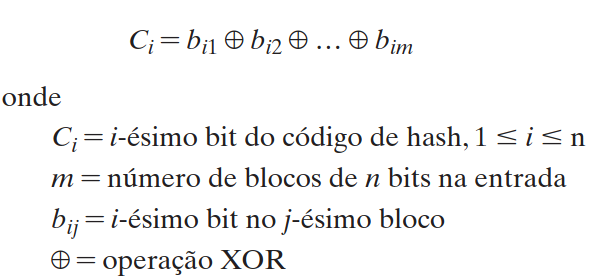
\includegraphics[width=0.5\linewidth]{Figuras/funcao-hash-simples.png}

\end{figure}

\end{frame}




\begin{frame}{Esquema de Hash simples com XOR}
    \centering
    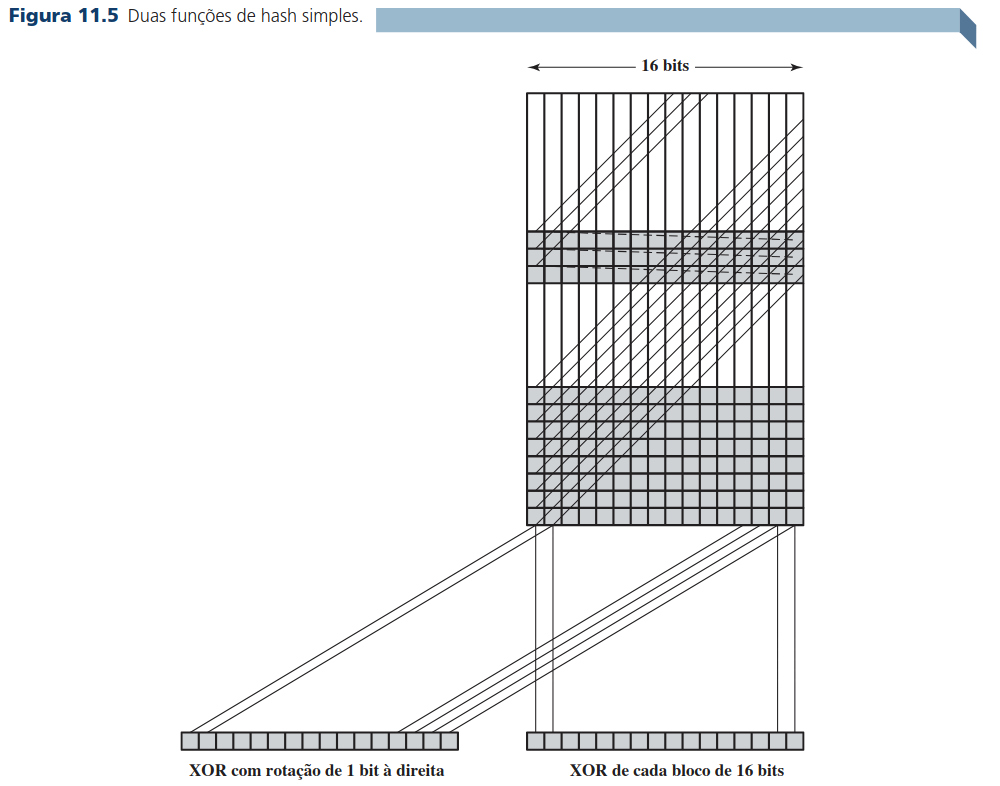
\includegraphics[width=0.65\linewidth]{Figuras/hash-simples-xor.png}
\end{frame}

\begin{frame}{Limitações do XOR em Funções de Hash}
    \begin{itemize}
        \item XOR simples não é suficiente quando apenas o código de hash é encriptado.
        \item Problema:  blocos de texto cifrado podem ser \textbf{reordenados} sem alterar o valor do hash.
        \item Isso permite que um atacante modifique a mensagem sem que a integridade seja detectada.
        \item Conclusão: para garantir a integridade, precisamos de funções de hash criptográficas \textbf{não lineares e resistentes a colisões}.
    \end{itemize}
\end{frame}

\begin{frame}{Pré-imagem e Colisões em Funções de Hash}
    \begin{itemize}
        \item Para um valor de hash $h = H(x)$, $x$ é chamado de \textbf{pré-imagem} de $h$.
        \item Isso significa que $x$ é um bloco de dados cuja função hash produz $h$.
        \item Funções hash são \textbf{mapas muitos-para-um}: para qualquer valor $h$, podem existir várias pré-imagens.
        \item Uma \textbf{colisão} ocorre se existirem $x \neq y$ tal que $H(x) = H(y)$.
        \item Colisões são indesejáveis quando funções de hash são usadas para \textbf{integridade de dados}.
    \end{itemize}
\end{frame}

\begin{frame}{Pré-imagens e Potenciais Colisões}
    \begin{itemize}
        \item Suponha uma função de hash $H$ com saída de $n$ bits e entrada de $b$ bits ($b > n$).
        \item Total de mensagens possíveis: $2^b$.
        \item Total de valores de hash possíveis: $2^n$.
        \item Em média, cada valor de hash corresponde a $2^{b-n}$ pré-imagens.
        \item Se $H$ distribui uniformemente os valores de hash, cada hash terá aproximadamente $2^{b-n}$ pré-imagens.
        \item Para entradas de tamanho variável, a variação de pré-imagens por valor de hash aumenta.
        \item Apesar disso, os riscos de segurança não são tão graves; é necessário definir requisitos precisos de segurança para funções de hash criptográficas.
    \end{itemize}
\end{frame}

\begin{frame}{Requisitos de Funções de Hash}
    
\begin{figure}
    \centering
    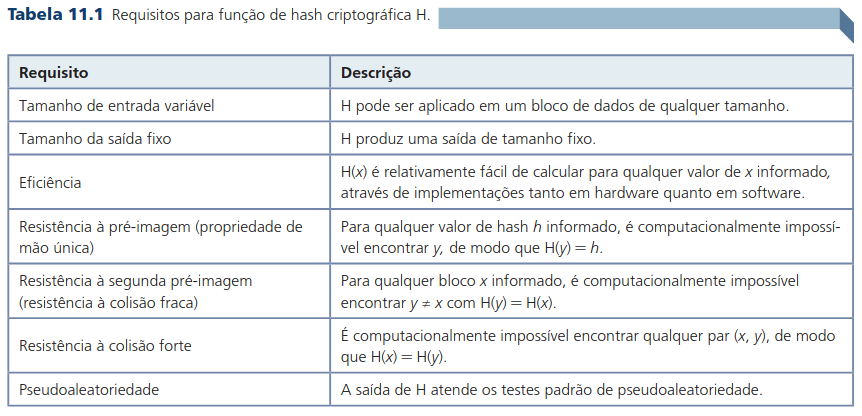
\includegraphics[width=0.9\linewidth]{Figuras/requisitos-funcao-hash.png}

\end{figure}
As primeiras três
propriedades são requisitos para a aplicação prática de uma função de hash.
\end{frame}

\begin{frame}{Resistência à Pré-imagem (Propriedade de Mão Única)}
    \begin{itemize}
        \item A resistência à pré-imagem significa que é fácil gerar o código de hash a partir da mensagem.
        \item Porém, é praticamente impossível gerar a mensagem a partir do código de hash.
        \item Essencial quando a autenticação envolve um valor secreto que não é transmitido.
        \item Se a função de hash não tiver esta propriedade, um invasor pode:
        \begin{itemize}
            \item Observar a mensagem $M$ e o hash $h = H(S || M)$.
            \item Inverter a função de hash para obter $S || M = H^{-1}(h)$.
            \item Recuperar o valor secreto $S$ facilmente.
        \end{itemize}
        \item Portanto, a resistência à pré-imagem é crucial para proteger valores secretos.
    \end{itemize}
\end{frame}

\begin{frame}{Resistência à Segunda Pré-imagem}
    \begin{itemize}
        \item Garante que é impossível encontrar uma mensagem alternativa com o mesmo valor de hash de uma mensagem específica.
        \item Importante para prevenção contra falsificação quando se usa um hash encriptado.
        \item Se a função de hash não possuir essa propriedade, um invasor poderia:
        \begin{itemize}
            \item Observar ou interceptar uma mensagem com seu hash encriptado.
            \item Decriptar o hash da mensagem original.
            \item Criar uma nova mensagem diferente com o mesmo hash.
        \end{itemize}
        \item Portanto, esta propriedade protege contra ataques de falsificação.
    \end{itemize}
\end{frame}

\begin{frame}{Funções Hash Fraca e Forte}
    \begin{itemize}
        \item Uma função de hash que satisfaz as primeiras cinco propriedades é chamada de \textbf{função hash fraca}.
        \item Se a função também satisfaz a sexta propriedade, \textbf{resistência à colisão}, é chamada de \textbf{função hash forte}.
        \item Função hash forte protege contra ataques onde terceiros tentam gerar mensagens diferentes com o mesmo hash.
        \item Exemplo de ataque sem resistência à colisão:
        \begin{itemize}
            \item Bob cria duas mensagens diferentes com o mesmo hash (m1 e m2).
            \item Alice assina a mensagem m1.
            \item Bob usa o hash da mensagem m1 para reivindicar que a mensagem m2 foi assinada.
        \end{itemize}
        \item Portanto, a resistência à colisão é crucial para evitar falsificação de assinaturas.
    \end{itemize}
\end{frame}

\begin{frame}{Pseudoaleatoriedade em Funções de Hash Criptográficas}
    \begin{itemize}
        \item A pseudoaleatoriedade não é tradicionalmente citada como requisito formal, mas é implicitamente importante.
        \item Funções de hash criptográficas são frequentemente usadas para:
        \begin{itemize}
            \item Derivação de chaves.
            \item Geração de números pseudoaleatórios (PRNG/PRF).
        \end{itemize}
        \item Nas aplicações de integridade de mensagens, as propriedades de resistência dependem de a saída parecer aleatória.
        \item Portanto, é apropriado considerar que uma função de hash produz uma saída pseudoaleatória.
    \end{itemize}
\end{frame}

\begin{frame}{Relação entre propriedades de Funções de Hash}
    
\begin{figure}
    \centering
    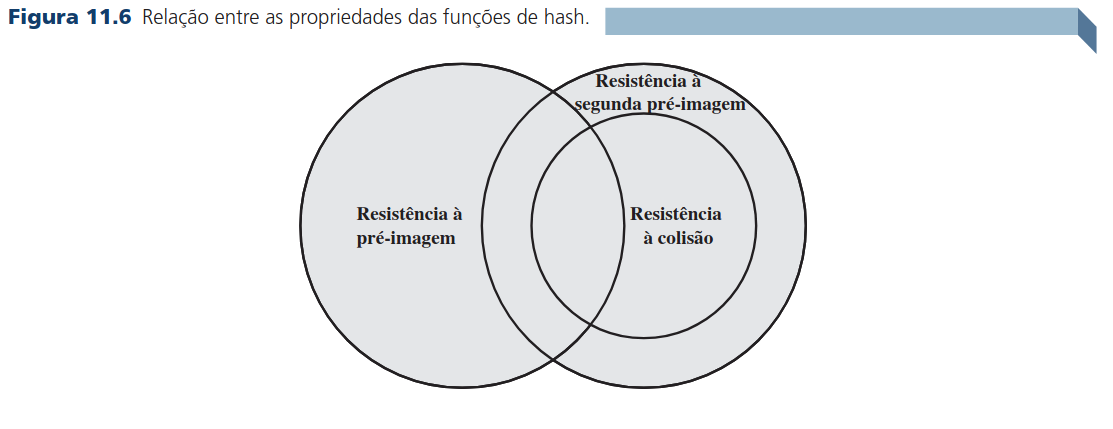
\includegraphics[width=0.9\linewidth]{Figuras/relacao-entre-propriedades-hash.png}

\end{figure}
\begin{itemize}


    \item  Uma função que é resistente à colisão também é resistente à segunda pré-imagem, mas o inverso não é necessariamente verdadeiro.
    \item Uma função pode ser resistente à colisão, mas não ser resistente à pré-imagem, e vice-versa. Uma função pode ser resistente à pré-imagem, mas não ser resistente à segunda pré-imagem e vice-versa.
    \end{itemize}
\end{frame}


\begin{frame}{Propriedades de resistência Funções de Hash e seu uso}
    
\begin{figure}
    \centering
    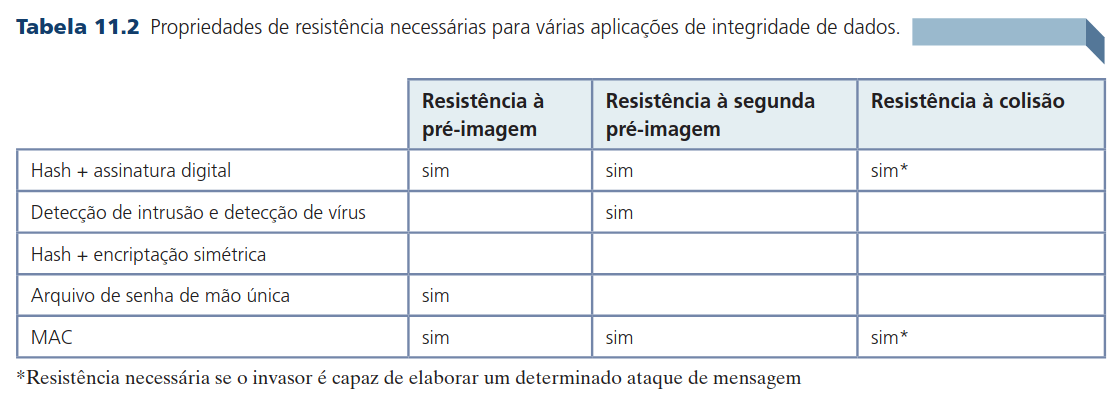
\includegraphics[width=\linewidth]{Figuras/propriedades-resistencia-hash.png}

\end{figure}
\end{frame}

\begin{frame}{Ataques de Força Bruta em Funções de Hash}
    \begin{itemize}
        \item Ataques de força bruta não dependem do algoritmo de hash, apenas do tamanho do valor de hash em bits.
        \item Consiste em tentar todas as combinações possíveis até encontrar uma pré-imagem ou colisão.
        \item O esforço necessário cresce exponencialmente com o tamanho do hash: para um hash de \(n\) bits, há \(2^n\) possíveis valores.
        \item Diferente da criptoanálise, que explora vulnerabilidades específicas do algoritmo.
        \item Exemplo: para um hash de 128 bits, seriam necessárias \(2^{128}\) tentativas em média para encontrar uma colisão por força bruta.
    \end{itemize}
\end{frame}
\begin{frame}{Ataques de Pré-imagem e Segunda Pré-imagem}
\textbf{Cenário}: O atacante conhece uma saída da Hash
    \begin{itemize}
        \item O adversário busca um valor \(y\) tal que \(H(y) = h\), onde \(h\) é um hash conhecido.
        \item Método de força bruta: testar valores aleatórios de \(y\) até encontrar uma correspondência.
        \item Para um hash de \(m\) bits, o esforço médio necessário é \(2^{m-1}\) tentativas.
        \item Esse ataque explora a dificuldade de inverter a função de hash (resistência à pré-imagem).
    \end{itemize}
\end{frame}
\begin{frame}{Ataques Resistentes à Colisão}
\textbf{Cenário}: O atacante busca desobrir pares de saída da Hash
    \begin{itemize}
        \item O adversário busca duas mensagens \(x\) e \(y\) tal que \(H(x) = H(y)\).
        \item Esse ataque exige \textbf{menos esforço} do que um ataque de pré-imagem ou segunda pré-imagem.
        \item Baseado no \textbf{paradoxo do aniversário}: a probabilidade de colisão aumenta rapidamente com o número de tentativas.
        \item Para um hash de \(m\) bits, o esforço médio para encontrar uma colisão é aproximadamente \(2^{m/2}\) tentativas.
    \end{itemize}
\end{frame}
\begin{frame}{Ataque de Colisão Explorado via Paradoxo do Aniversário}
Estratégia para explorar o paradoxo do dia do aniversário:
    \begin{itemize}
        \item Preparação da origem A: mensagem legítima \(x\) é criada
        \item Oponente gera \(2^{m/2}\) variações \(x'\) de \(x\) com mesmo significado e armazena os hashes.
        \item Oponente prepara uma mensagem fraudulenta \(y\) para a qual deseja a assinatura.
        \item Pequenas variações \(y'\) de \(y\) são geradas; o oponente calcula \(H(y')\) e verifica correspondência com algum \(H(x')\).
        \item Quando há correspondência, a variação válida de A é usada para assinatura, que é então aplicada à variação fraudulenta \(y'\). 
    \end{itemize}
    Ambas produzem a mesma assinatura.
\end{frame}
\begin{frame}{Exemplo de Ataque de Colisão com Hash de 64 bits}
    \begin{itemize}
        \item Com um hash de 64 bits, o esforço necessário é da ordem de \(2^{32}\).
        \item Criação de variações que mantêm o mesmo significado não é difícil.
        \item Exemplos de variações:
        \begin{itemize}
            \item Inserção de pares de caracteres ``espaço-espaço-retrocesso'' entre palavras.
            \item Substituição de ``espaço-retrocesso-espaço'' em posições selecionadas.
            \item Reescrita da mensagem mantendo o significado original.
        \end{itemize}
    \end{itemize}
\end{frame}
\begin{frame}{Resumo do esforço exigido}
    \textbf{Resumo}: Para um código de hash de tamanho m, o nível de esforço exigido, conforme vimos, é proporcional ao seguinte:
    \begin{figure}
        \centering
        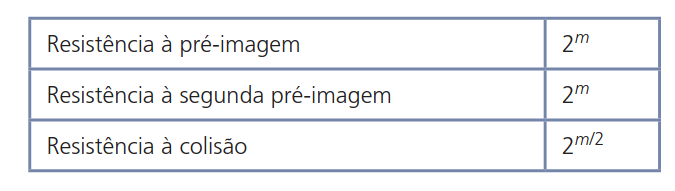
\includegraphics[width=0.7\linewidth]{Figuras/resumo-do-esforco-exigido.png}
    \end{figure}
\end{frame}
\begin{frame}{Resistência a Colisões em Hashes}
    \begin{itemize}
        \item A resistência à colisão é desejável em códigos de hash seguros.
        \item Para um hash de $m$ bits, a força contra ataques por força bruta é aproximadamente $2^{m/2}$.
        \item Van Oorschot e Wiener [VANO94] projetaram uma máquina de US\$10 milhões para MD5 (128 bits):
            \begin{itemize}
                \item Capaz de encontrar uma colisão em 24 dias.
                \item Mostra que 128 bits é inadequado para segurança moderna.
            \end{itemize}
        \item Hashes de 160 bits (como SHA-1) aumentam a resistência:
            \begin{itemize}
                \item Mesma máquina levaria mais de 4.000 anos para encontrar uma colisão.
                \item Contudo, com tecnologia atual, 160 bits começa a ficar suspeito.
            \end{itemize}
        
    \end{itemize}
\end{frame}

\begin{frame}{Criptoanálise de Funções de Hash e MACs}
    \begin{itemize}
        \item Assim como em algoritmos de criptografia, ataques criptoanalíticos em \textbf{hashes} e \textbf{MACs} buscam explorar propriedades do algoritmo para superar a simples busca exaustiva.
        \item A resistência de um hash ou MAC à criptoanálise é medida comparando-se seu esforço com o esforço de um ataque por força bruta.
        \item Um hash ou MAC ideal exigirá \textbf{esforço criptoanalítico maior ou igual ao esforço por força bruta}.
    \end{itemize}
\end{frame}
\begin{frame}{Estrutura Iterativa de Funções de Hash}
    \begin{itemize}
        \item A estrutura iterativa de hash foi proposta por Merkle [MERK79, MERK89] e é usada na maioria das funções de hash atuais, incluindo SHA.
        \item Funcionamento geral:
        \begin{itemize}
            \item A mensagem de entrada é dividida em $L$ blocos de tamanho fixo $b$ bits.
            \item Se necessário, o bloco final é preenchido para completar $b$ bits e inclui o tamanho total da mensagem.
            \item Incluir o tamanho dificulta ataques, pois o oponente deve encontrar colisões com mensagens do mesmo ou de tamanhos diferentes que levem ao mesmo hash.
        \end{itemize}
        \item O algoritmo usa repetidamente uma \textbf{função de compactação} $f$:
        \begin{itemize}
            \item Recebe duas entradas: a \textbf{variável de encadeamento} (n bits da etapa anterior) e o bloco atual (b bits). Normalmente, b $>$ n;
            \item Produz uma saída de $n$ bits.
            \item A variável de encadeamento inicial é definida pelo algoritmo e o valor final dela é o \textbf{hash resultante}.
        \end{itemize}
    \end{itemize}
\end{frame}

\begin{frame}{Estrutura geral de hash seguro}
       \begin{figure}
        \centering
        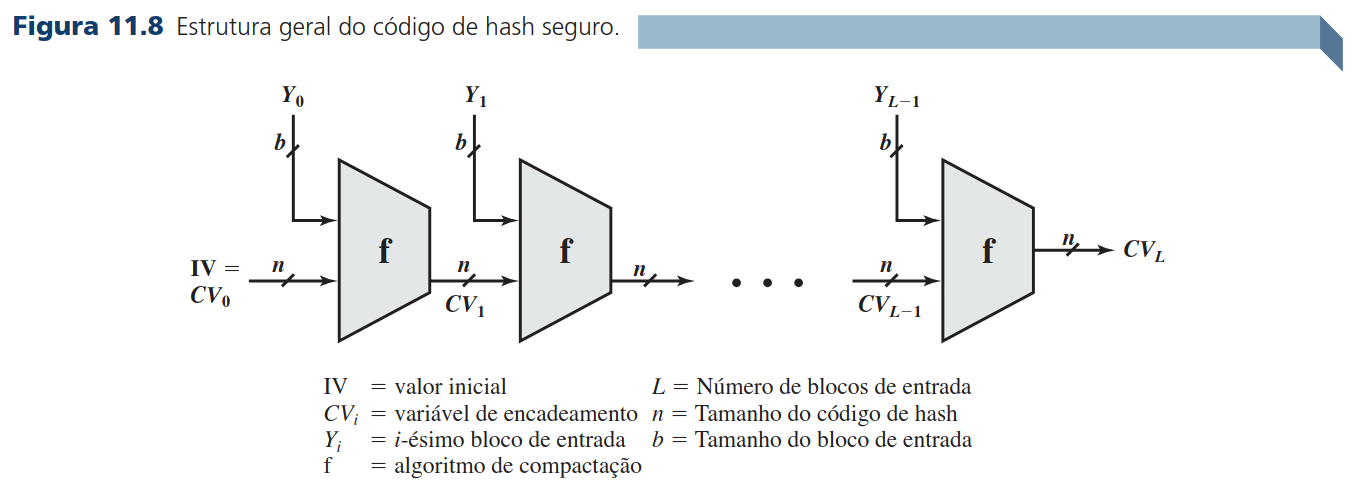
\includegraphics[width=0.9\linewidth]{Figuras/estrutura-gera-hash-seguro.png}
    \end{figure}
\end{frame}

\begin{frame}{Estrutura geral de hash seguro}
       \begin{figure}
        \centering
        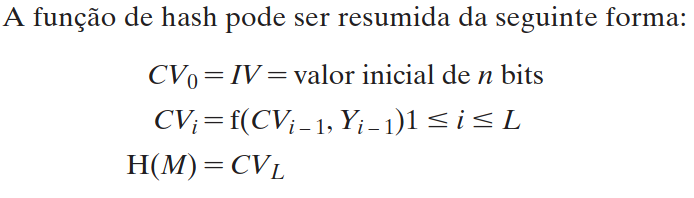
\includegraphics[width=0.9\linewidth]{Figuras/pode-ser-resumida-seg-forma.png}
    \end{figure}
onde a entrada da função de hash é uma mensagem M consistindo nos blocos Y0, Y1, ..., YL-1
\end{frame}

\begin{frame}{Motivação e Criptoanálise de Funções de Hash}
    \begin{itemize}
        \item Motivação da estrutura iterativa (Merkle [MERK89], Damgård [DAMG89]):
        \begin{itemize}
            \item Se a função de compactação $f$ for à prova de colisão, a função de hash iterativa resultante também será.
            \item Permite criar hashes seguros para mensagens de qualquer tamanho.
            \item O design seguro de uma função de hash se reduz ao design de uma função de compactação segura para blocos de tamanho fixo.
        \end{itemize}
        \item Criptoanálise de funções de hash:
        \begin{itemize}
            \item Foca na estrutura interna de $f$.
            \item Ataques procuram produzir colisões eficientes para uma única execução de $f$, considerando o valor fixo do IV.
            \item Normalmente, $f$ consiste em várias rodadas, e o ataque analisa padrões de mudança de bits entre rodadas.
        \end{itemize}
    \end{itemize}
\end{frame}

\begin{frame}{Colisões em Funções de Hash}
    \begin{itemize}
        \item \textbf{Importante}: Para qualquer função de hash, \textbf{colisões sempre existem}:
        \begin{itemize}
            \item Mensagens têm tamanho $\ge 2b$ (devido ao campo de tamanho)  
            \item Hashes têm tamanho fixo $n$, com $b > n$
        \end{itemize}
        \item O objetivo de uma função de hash segura não é eliminar colisões (isso é impossível),  
        mas torná-las \textbf{computacionalmente inviáveis de encontrar}.
        \item Assim, a segurança é definida pelo \textbf{esforço necessário para descobrir uma colisão}, não pela sua inexistência.
    \end{itemize}
\end{frame}

\begin{frame}{Secure Hash Algorithm (SHA)}
    \begin{itemize}
        \item O \textbf{SHA} é a função de hash mais utilizada nos últimos anos.
        \item Em 2005, era praticamente o último algoritmo de hash padronizado restante após vulnerabilidades em outros algoritmos.
        \item Desenvolvido pelo \textbf{NIST} e publicado como padrão federal (\textbf{FIPS 180}) em 1993.
        \item Primeira versão (\textbf{SHA-0}) apresentou vulnerabilidades criptoanalíticas.
        \item Revisão lançada em 1995 (\textbf{FIPS 180-1}), conhecida como \textbf{SHA-1}.
        \item Baseado na função de hash \textbf{MD4}, seguindo de perto seu projeto.
    \end{itemize}
\end{frame}

\begin{frame}{SHA-1 e SHA-2}
    \begin{itemize}
        \item \textbf{SHA-1} produz um hash de 160 bits.
        \item Em 2002, o \textbf{NIST} revisou o padrão (\textbf{FIPS 180-2}), definindo três novas versões:
        \begin{itemize}
            \item SHA-256 (256 bits)
            \item SHA-384 (384 bits)
            \item SHA-512 (512 bits)
        \end{itemize}
        \item Coletivamente, estas versões são conhecidas como \textbf{SHA-2}.
        \item Mantêm a mesma estrutura básica do SHA-1, usando aritmética modular e operações binárias lógicas.
        \item Em 2008, o \textbf{FIPS PUB 180-3} adicionou uma versão de 224 bits (SHA-224).
        \item SHA-1 e SHA-2 também são especificados no \textbf{RFC 6234}, que inclui implementação em C.
    \end{itemize}
\end{frame}

\begin{frame}{Descontinuação do SHA-1}
    \begin{itemize}
        \item Em 2005, o \textbf{NIST} anunciou a intenção de retirar a aprovação do SHA-1 e adotar o SHA-2 por volta de 2010.
        \item Uma equipe de pesquisa demonstrou um ataque que poderia gerar duas mensagens diferentes com o mesmo hash SHA-1 usando $2^{69}$ operações.
        \item Este número é significativamente menor que as $2^{80}$ operações anteriormente estimadas para encontrar uma colisão.
        \item O resultado acelerou a necessidade de transição para SHA-2.
        \item Referência: Wang et al. [WANG05].
    \end{itemize}
\end{frame}

\begin{frame}{Tabela SHA}
\begin{figure}
    \centering
    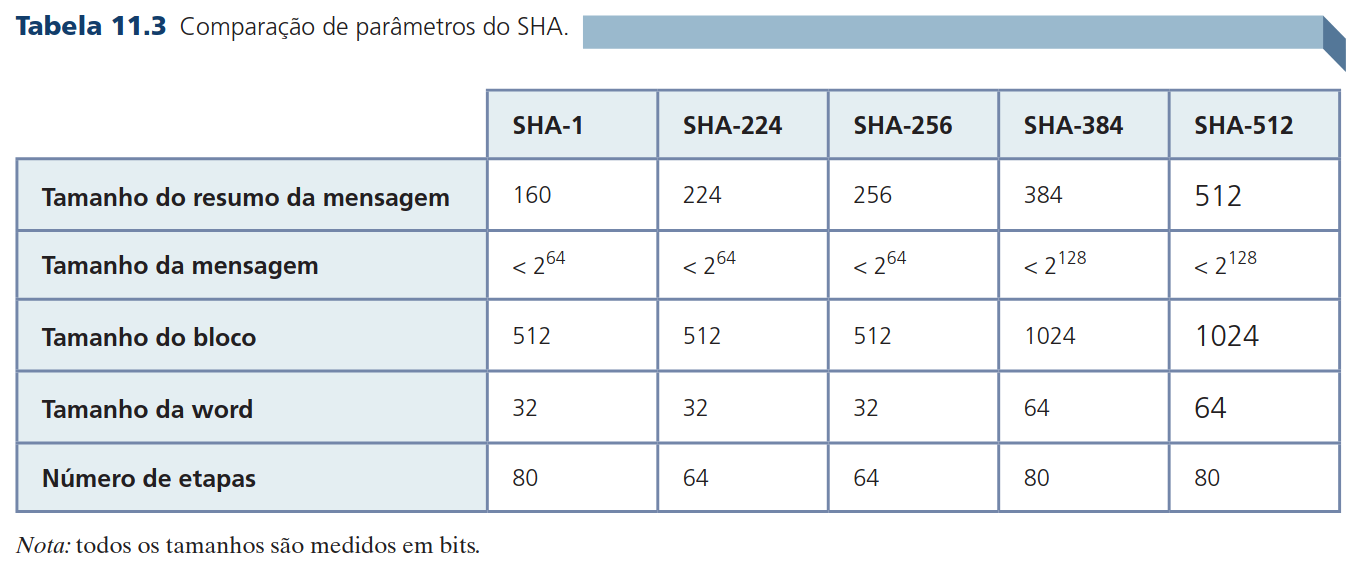
\includegraphics[width=\linewidth]{Figuras/tabela-sha.png}

\end{figure}
    
\end{frame}

\begin{frame}{SHA-512: Etapa 1 -  Preenchimento}
    \begin{itemize}
        \item Entrada: mensagem com tamanho menor que $2^{128}$ bits.
        \item Saída: resumo (hash) de 512 bits.
        \item Processamento em blocos de 1024 bits.
        \item \textbf{Etapa 1 - Preenchimento:}
        \begin{itemize}
            \item A mensagem é preenchida para que o tamanho seja congruente a 896 módulo 1024.
            \item O preenchimento é sempre aplicado, mesmo se a mensagem já tiver o tamanho desejado.
            \item Número de bits de preenchimento: entre 1 e 1024.
            \item Estrutura do preenchimento: um bit 1 seguido pelos bits 0 necessários.
        \end{itemize}
    \end{itemize}
\end{frame}

\begin{frame}{SHA-512: Etapa de Anexar Tamanho}
    \begin{itemize}
        \item \textbf{Etapa 2 - Anexar tamanho:}
        \begin{itemize}
            \item Um bloco de 128 bits é anexado à mensagem.
            \item O bloco contém o tamanho da mensagem original (antes do preenchimento) como um inteiro de 128 bits sem sinal.
            \item Ordem dos bytes: byte mais significativo primeiro.
        \end{itemize}
        \item Após as duas primeiras etapas, a mensagem resultante tem comprimento múltiplo de 1024 bits.
        \item Mensagem expandida representada como blocos de 1024 bits: $M_1, M_2, \dots, M_N$.
        \item Tamanho total da mensagem expandida: $N \times 1024$ bits.
    \end{itemize}
\end{frame}

\begin{frame}{SHA-512: Inicialização do Buffer de Hash}
    \begin{itemize}
        \item Um buffer de 512 bits mantém resultados intermediários e finais.
        \item Representado por 8 registradores de 64 bits: $a, b, c, d, e, f, g, h$.
        \item Inicialização com valores hexadecimais:
\begin{figure}
    \centering
    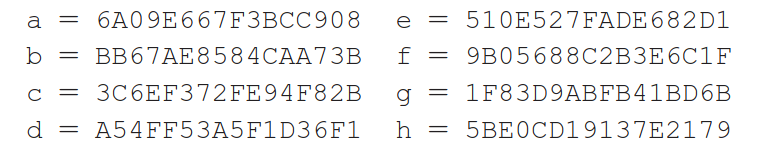
\includegraphics[width=\linewidth]{Figuras/buffer-hash-sha256.png}

\end{figure}
        \item Valores armazenados em \textbf{big-endian}.
        \item Derivados dos primeiros 64 bits das partes fracionárias das raízes quadradas dos oito primeiros números primos.
    \end{itemize}
\end{frame}
